\documentclass{article}
\usepackage{ucs}
\usepackage[utf8x]{inputenc} % Включаем поддержку UTF8
\usepackage[russian]{babel}  % Включаем пакет для поддержки русского языка}
\usepackage{url}
\usepackage{enumerate}
\usepackage{graphicx}


\title{Задача о пьянице}
\author{Баранов Александр}
\date{} 

\pagestyle{plain}

\begin{document}
 
    \begin{titlepage}
    \begin{center}
        \large{МОСКОВСКИЙ ГОСУДАРСТВЕННЫЙ УНИВЕРСИТЕТ\\
        имени М. В. ЛОМОНОСОВА\\
        \underline{\hspace{\textwidth}}
        ФИЗИЧЕСКИЙ ФАКУЛЬТЕТ}\\
        
        \vspace{30pt} %отступ перед        

        Курсовая работа по дисциплине\\
        ``Параллельное программирование''

        \vspace{100pt} %отступ перед

        \Large{Задача по пьянице}

        \vspace{100pt} %отступ после
    \end{center}
    
        \begin{flushright}
            \large{Выполнил\\
            студент 2 курса группы 213\\
            Баранов Александр Сергеевич\\
            \underline{\hspace{14em}}\\
            «\underline{\hspace{1em}}»\underline{\hspace{10em}} 2012\\
            }
            \vspace{50pt}
            \large{Научный руководитель\\
            Никитин Николай Викторович\\
            \underline{\hspace{14em}}\\
            «\underline{\hspace{1em}}»\underline{\hspace{10em}} 2012
            }
        \end{flushright}
        
        %\vspace{10pt}
        %Допущена к защите "<\underline{\hspace{1em}}">\underline{\hspace{4em}} 2222 года\newline
        \vspace{10pt}
        %\begin{tabbing}
        %Заведующий кафедрой мистических процессов\qquad\= \qquad\= \qquad\= Научный руководитель\\
        %д.ф.-м.н., профессор \> \> \> д.ф.-м.н., профессор\\
        %\\
        %\underline{\hspace{4.5cm}}О.\,О. Вротмненогов \> \> \> \underline{\hspace{3.5cm}} Д.\,Д. Блэйн\\
        %\end{tabbing}
        
        \begin{center}
        \large{Москва, 2012}
        \end{center}
\end{titlepage}

\pagebreak
    
    
        
    \section{Введение}
        Задача о пьянице является частным случаем случайного блуждания \cite{wiki}, в котором условия завершения ведут к определённому конечному состоянию. (надо бы точнее перевести Drunkard's walk, a type of a random walk in which termination conditions lead to a biased ending state)

        Постановка задачи: пьяница выходит из бара и случайным образом «блуждает» по городу, представленному множеством перпендикулярно пересекающихся улиц, пока не доберётся до дома. На некоторых перекрёстках города стоят «полицейские». Когда пьяница попадает на перекрёсток с «полицейскими», его блуждание прекращается(он попадает в полицейский участок). Нужно определить, с какой вероятностью пьяница дойдёт от бара до дома при заданных параметрах города.

        Данная задача (несмотря на свою классическую постановку) относится к задачам на решение уравнения Шредингера со случайным потенциалом. Такая задача может описывать:
        \begin{enumerate}[a)]
            \item Распространение тока в проводнике или в кристалле с дефектами
            \item Измерение положения частицы и проблему редукции волновой функции
        \end{enumerate}

        Обобщение данной задачи на пространства с произвольной размерностью дает некоторые относительно простые параллели с результатами в теории струн. Кроме того, подобную задачу можно в упрощенной постановке решить аналитически.

        \begin{figure}[ht]
            \centering
            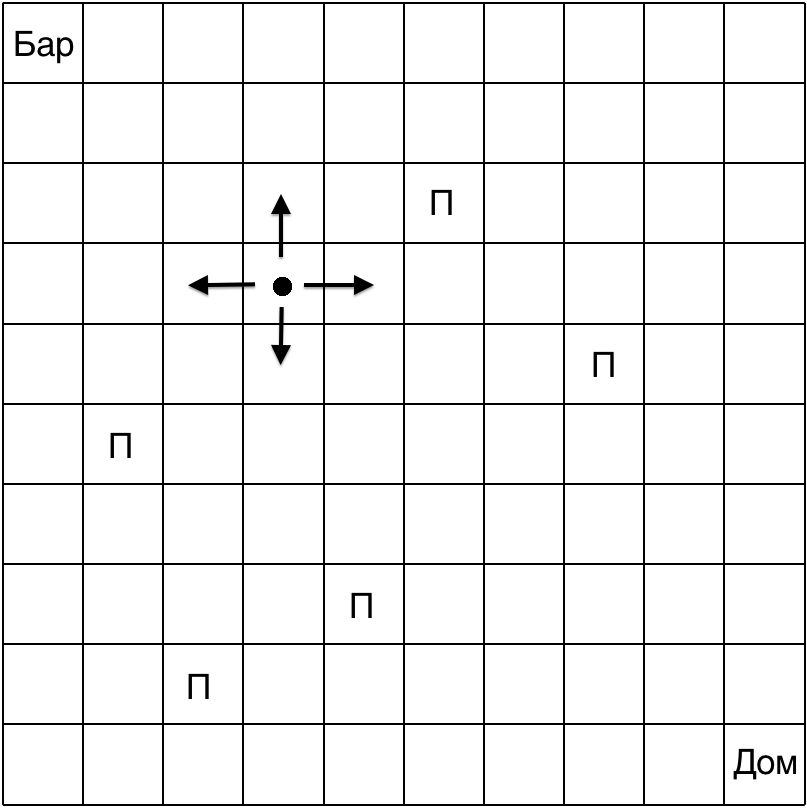
\includegraphics[width=7.5cm]{pict.png}
            \caption{Схематическая визуализация задачи}
        \end{figure}
    \pagebreak


    \section{Реализация}
    \subsection{Общие аспекты}

    Для решения поставленной задачи была написанна программа, проводящая симуляцию поведения пьяниц в городе. Для ускорения работы программы была использованна библиотека OpenMP. Выбор данной библиотеки связан с соображениями экономии памяти. Запуск симуляции в различных процессах(библиотека MPI) привёл бы к выделению дополнительной памяти в каждом процессе для каждой симуляции.

    С помощью аргументов командной строки, на вход программы подаются следующие параметры:
    \begin{enumerate}[1.]
        \item Размерность города (флаг -d)
        \item Размер города по каждому измерению (флаг -N)
        \item Количество «полицейских» (флаг -c)
        \item Количество регенераций «полицейских» в городе (флаг -K)
        \item Количество пьяниц на одну регенерацию (флаг -M)
    \end{enumerate}

    Подробнее о использовании этих параметров можно прочитать при вызове программы с флагом -h.

    На выходе выдаются данные в формате: \textit{C P SP T M K}, где:
    \begin{enumerate}[1.]
        \item C — количество полицейских
        \item P — измеренная вероятность
        \item SP — среднеквадратичное отклонение измеренной вероятности
        \item T — затраченное на выполнение время
        \item M — количество пьяниц на одну регенерацию
        \item K — количество регенераций за всю симуляцию.
    \end{enumerate}
    \pagebreak

    \subsection{Параллелизация и общая схема работы}
    «Город» представлен в программе многомерным массивом grid, состоящий из $N^{d}$ элементов, использующимся как одномерный, в связи с динамичностью задания его размерности.

    Основным в программе является цикл симуляций, состоящий из K итераций.
    Распишем алгоритм работы каждой итерации:
    \begin{enumerate}[1.]
        \item Массив grid сбрасывается в значение 0(регенерируется) вызовом memset. Далее случайным образом некоторым(в количестве C) его элементам присваивается значение 1, означая наличие полицейского на данном перекрёстке.
        \item Запускается несколько потоков(их число берётся из переменной окружения \textit{OMP\_NUM\_THREADS}), в каждом из которых происходит симуляция блуждания $\frac{M}{OMP\_NUM\_THREADS}$ пьяниц от точки с координатами $(0, 0 … 0)$ до точки с координатами $(N, N … N)$. Данные о прошедших пьяницах записываются в массив stats, общий для всех потоков.
    \end{enumerate}

    Регенерация сетки была сделана для точности определения вероятности. Если бы симуляция проводилась на одной сетке, то была бы вероятность получать «плохое» расположение «полицейских» — расположение, при котором полицейские полностью блокировали бы любой путь от бара до дома. См. Рисунок 2
    \begin{figure}[ht]
        \centering
        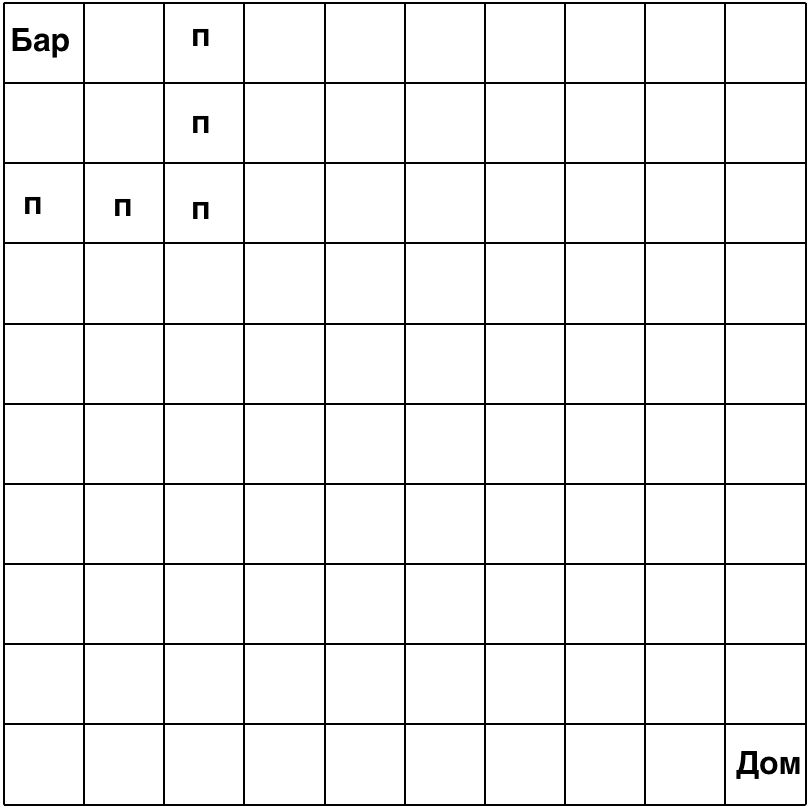
\includegraphics[width=6cm]{pict2.png}
        \caption{«Плохое» расположение}
    \end{figure}


    При записи в массив stats может создаться состояние гонки\cite{wikirc}, особенно, когда количество полицейских $C = 1$. По этому запись в массив stats была сделанна атомарно по средствам директивы OpenMP atomic.
    \pagebreak

    \section{Результаты}
    \subsection{Общие результаты}
    Общий вид зависимости вероятности прохождения от количества «полицейских» приведён на Рисунке 3 для сетки 10x10x10.

    \begin{figure}[ht]
        \centering
        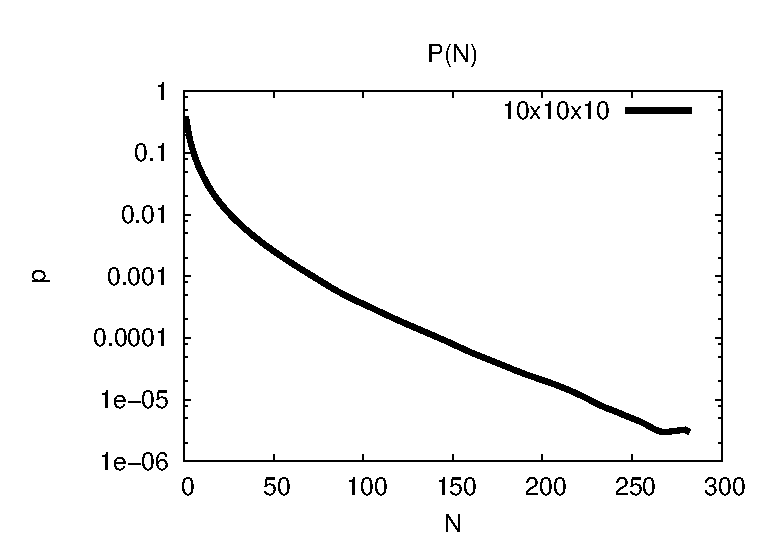
\includegraphics[scale=0.6]{1.eps}
        \caption{Зависимость для сетки 10x10x10}
    \end{figure}
    
    Неровность в конце графика не является значительной, так как соответствует значениям, для которых стандартное отклонение больше самой величины вероятности. Здесь стоит отметить, что увеличение параметров M и K ведут к уменьшению стандартного отклонения при измерении вероятностей, в то же время увеличивая время симуляции.

    На Рисунке 4 показанны зависимости для различных сеток.

    \begin{figure}[ht]
        \centering
        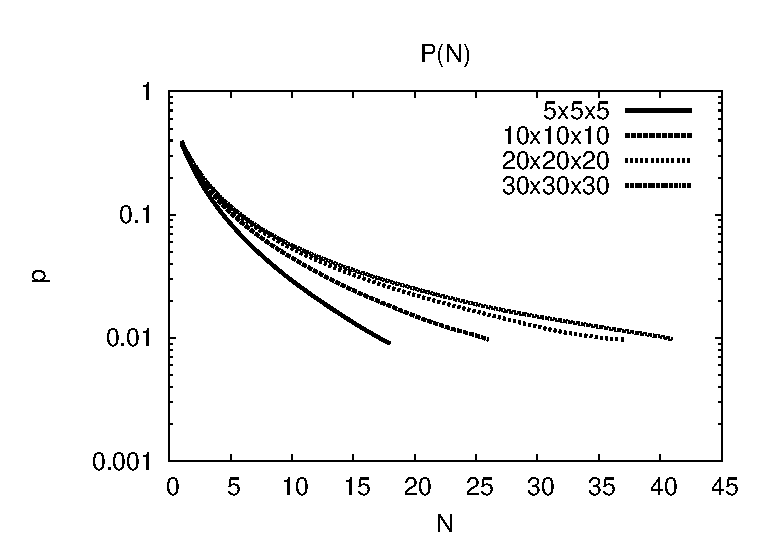
\includegraphics[scale=0.6]{2.eps}
        \caption{Зависимость для нескольких сеток}
    \end{figure}

    \pagebreak

    \subsection{Ускорение}
    Для теста ускорения работы программы были выбраны следующие параметры:
    $$dim = 3;  N = 10;  C = 10;  M = 100000;  K = 1000$$

    Зависимость времени выполнения от количества потоков представлена на Рисунке 5. Тестирование проводилось на 4-х ядерном процессоре Intel Core i5 2.8 ГГц(8 МБ L3, 256 КБ L2).
    \begin{figure}[ht]
        \centering
        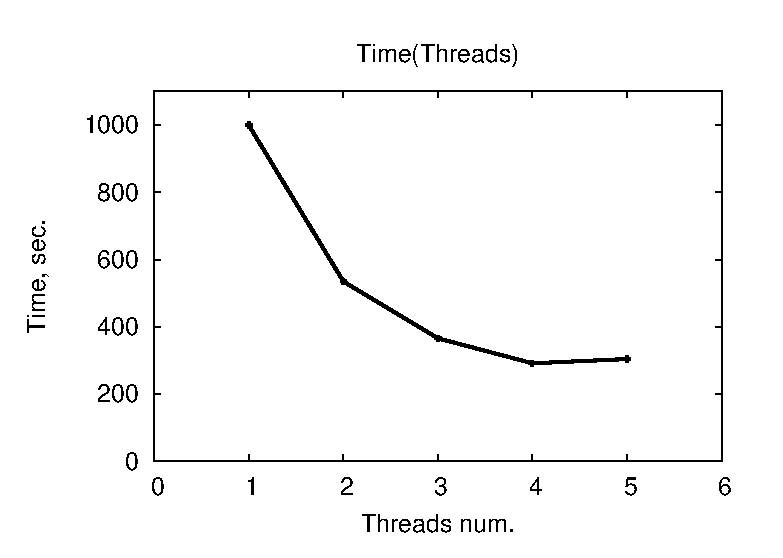
\includegraphics[scale=0.75]{3.eps}
        \caption{Зависимость времени от количества процессов}
    \end{figure}

    \pagebreak

    \section{Выводы}
    В данной курсовой работе для изучение «Задачи о пьянице» была написанна программа, производящая симуляцию данной задачи. Было изучено распределение вероятностей в задаче, а также исследовано ускорение в зависимости от количества потоков.
    \pagebreak

    \begin{thebibliography}{9}
    \bibitem{tale}
        Drunkard and Policemen
        \emph{\url{http://www.tcm.phy.cam.ac.uk/~dek12/tales/Tale-04.pdf}}

    \bibitem{wiki}
      Wikipedia — Random-Walk,
      \emph{\url{http://en.wikipedia.org/wiki/Random_walk}}.

    \bibitem{wikirc}
      Wikipedia — Race condition,
      \emph{\url{http://en.wikipedia.org/wiki/Race_condition}}.

    \bibitem{openmp}
      OpenMP 3.1 Specifications,
      \emph{\url{http://www.openmp.org/mp-documents/OpenMP3.1.pdf}}.
      
    \end{thebibliography}

\end{document}